\chapter{Ein Kapitel}
\label{cha:grafiken}
Hier kommt eine kurze Zusammenfassung des Kapitels hin. 

\section{Bilder}
\label{sec:bilder}

In Abbildung~\ref{fig:bild1-und-bild2} findet man ein  sch{\"o}nes Beispiel f{\"u}r das  Paket subfigure. Subfigure ist sehr praktisch beim Setzen von mehreren Bildern in ein Bild. Man beachte, dass man mit dem Befehl ref auf Bilder verweisen kann, wenn diesen mit dem Befehl label eine Marke zugewiesen wurde. Nicht alle Dateiformate können so problemlos wie ``.eps'' mit Latex direkt eingebunden werden. Benötigt man zum Beispiel eine pdf Grafik, so kann man das Dokument mit pdflatex compilieren. Hat man alle Bilder sowohl als pdf als auch als eps, kann man wahlweise latex oder pdflatex nutzen. Ansonsten hilft auch zeitweiliges auskommentieren der Bilder.


Zum Zeichnen von plots ist gnuplot sehr zu empfehlen (vgl. Abbildung \ref{fig:bild1}). Ist perfekt f{\"u}r zwei oder dreidimensionale Plots und schaut um Welten besser aus als Excel.

Zum Malen von Bildern ist das Programm xfig oder jfig sehr gut geeignet (vgl. Abbildung \ref{fig:bild2}). Schaut zwar am Anfang ein bi{\ss}chen seltsam aus, ist aber sehr m{\"a}chtig.

\begin{figure}
\centering
\subfigure[Ein mit gnuplot erzeugtes Bild\label{fig:bild1}]
        {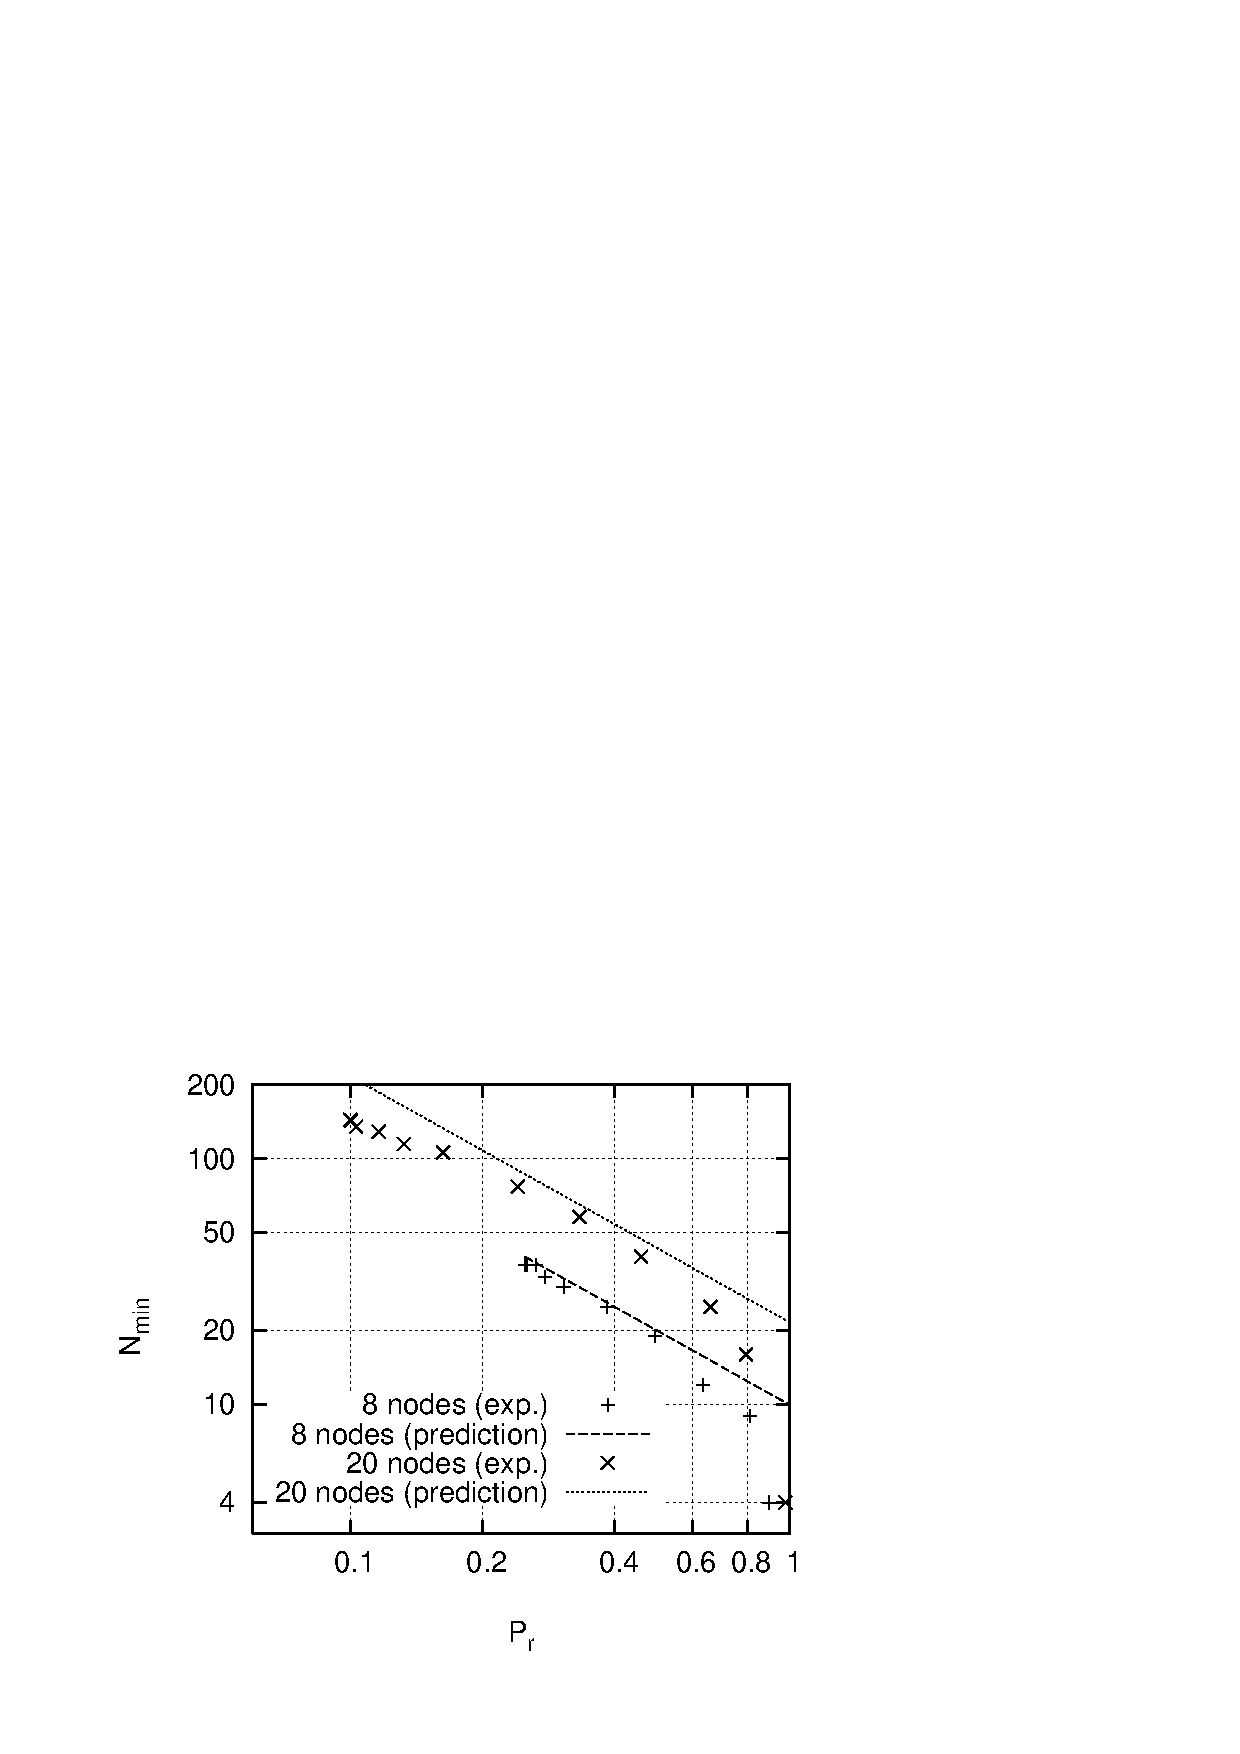
\includegraphics[width=\columnwidth]{grafiken/n-over-r8-20}
        }
\subfigure[Ein mit xfig erzeugtes Bild\label{fig:bild2}]
        {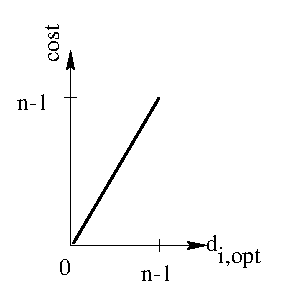
\includegraphics[width=3cm]{grafiken/cost}} 
\caption[Das hier steht im Abbildungsverzeichnis.]{Beispiele f{\"u}r sch{\"o}ne Bilder.\label{fig:bild1-und-bild2}}

\end{figure}


\section{Editor}

Als Editor f{\"u}r Fortgeschrittene ist xemacs gut geeignet.
Bei Verwendung von xemacs ist der Gebrauch der reftex und auctex-pakete zu empfehlen.
Als Rechtschreibprogramm sollte aspell verwendet werden und folgender Code in init.el eingef{\"u}gt werden.


 (require 'iso-cvt)\\
  (add-hook 'LaTeX-mode-hook\\
    (function (lambda ()\\
      ;; Setze Anfuehrungszeichen etc. fuer Style german\\
      (TeX-run-style-hooks "german")\\
      ;;\\
      ;; Lade Buffer und wandle nach ISO Latin-1:\\
      (format-encode-buffer 'plain)\\
      )))\\
\\
      (setq ispell-silently-savep t) ;save new words in pdict without questioning\\
(setq ispell-help-in-bufferp 'electric) ;get a better help buffer\\
(setq ispell-program-name "aspell")\\
(setq ispell-extra-args '("-W" "2"))\\
\\
(column-number-mode t)\\
\\
(custom-set-variables\\
 '(paren-mode 'sexp nil (paren)))\\
\\
 (setq reftex-plug-into-AUCTeX t)\\
(require 'reftex "reftex" t)\\
 (turn-on-reftex) ; use reftex\\
\\
 


Neulinge k{\"o}nnen auch einen sonstigen Editor oder Sachen wie Texnic Center, etc verwenden.

\section{Mathematik}

In latex kann man Formeln wundersch{\"o}n setzen.

\selectlanguage{english} % The following chapter is in english
As the following stuff is in English, we must change the hyphenation style.


The OCST problem is defined as follows. Let $G=(V,E)$ be a connected, undirected graph with $n=|V|$ nodes and $m=|E|$ edges. There are  communication, or transportation demands, between every pair of nodes.  An $n \times n$ {\em demand matrix} $R=(r_{ij})$ specifies the demands, where $r_{ij}$ is the amount of traffic required between location $v_i$ and $v_j$. Similarly, an $n\times n$ {\em distance matrix} $W=w_{ij}$ determines the distance weights between each pair of sites. 
A tree $T=(V,F)$ where $F \subseteq E$ and $|F|=|V|-1$ is called a {\em spanning tree} of $G$ if it connects all the nodes. The weight $w(T)$ of the spanning tree is the weighted sum over all pairs of vertices of the cost of the path between the pair in $T$. The communication cost over the tree $T$ is defined as 
\begin{equation}
  \label{equ:1}
w(T)=\sum_{i,j\in V}w_{ij}b_{ij},
\end{equation}
where $B=b_{ij}$ denotes the traffic flowing directly and indirectly across the edge connecting nodes $i$ and $j$. It is calculated according to the structure of $T$. 
$T$ is the optimal communication spanning tree if $w(T)\leq w(T')$ for all other spanning trees $T'$. %For the experiments we assume that there is an unique optimum tree ($w_{ij}\neq w_{kl}\forall (i\neq k, j\neq l)$).
The OCST problem becomes the minimum spanning tree (MST) problem if $w(T)=\sum_{i,j\in V}w_{ij}$. Then, $T$ is the simple minimum spanning tree if $w(T)\leq w(T')$  for all other spanning trees $T'$.%, where $w(T)=\sum_{i,j\in V}w_{ij}$. 
%In most instances of the OCST problem, the cost $f(w_{ij},b_{ij})$ of each link connecting the nodes $i$ and $j$ is calculated as the product of the distances $w_{ij}$ times the overall traffic $b_{ij}$ running over the link, so that $f=w_{ij}b_{ij}$. 

Cayley's formula identifies the number of spanning trees on $n$ nodes as $n^{n-2}$ . Furthermore, there are $n$ different stars on a graph of $n$ nodes. The similarity between two spanning trees $T_i$ and $T_j$ can be measured using the distance   $d_{ij}\in\{0,1,\ldots,n-1\}$ as 
$$
d_{ij}=\frac{1}{2}\sum_{u,v\in V,u<v}|l^{i}_{uv}-l^{j}_{uv}|,
$$
where $l^{i}_{uv}$ is 1 if an edge from $u$ to $v$ exists in $T_i$ and 0 if it does not exist in $T_i$. The number of edges that two trees $T_i$ and $T_j$ have in common is $n-1-d_{ij}$.




\selectlanguage{ngerman} % deutsch

Ab jetzt wieder deutsche Trennung.

In Abbildung \ref{fig:2dnorm} gibt es noch ein Beispiel f{\"u}r ein Bild und in Tabelle \ref{tab:einfache-tabelle} gibt es ein einfaches Bild. Tabelle~\ref{tab8:results-testproblem-deceptive} stellt eine etwas kompliziertere Tabelle dar. 
\begin{figure}[htb]
        \begin{center}
        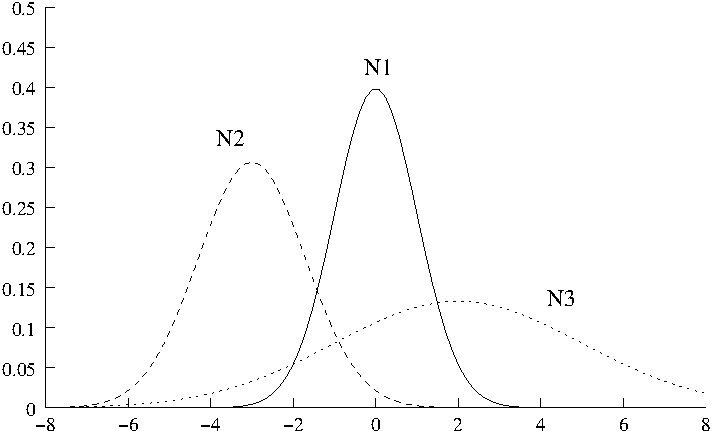
\includegraphics[width=8cm]{grafiken/norm_uni}
        \caption{Dichten univariater Normalverteilungen}
        \label{fig:2dnorm}
        \end{center}
\end{figure}


Beim Aufbau von Kommunikationsnetzen stehen Unternehmen vor dem Problem, eine Menge von unterschiedlichen Standorten so durch Leitungen zu verbinden, dass bestimmte Qualit{\"a}tsanforderungen (z.B. Sicherheit, Bandbreite, Zu\-ver\-l{\"a}ssig\-keit, Skalierbarkeit, etc.) eingehalten werden und gleichzeitig die Netzstruktur so gew{\"a}hlt wird, dass die Kosten des Netzaufbaus minimiert werden. Unternehmen, f{\"u}r welche der Aufbau von Kommunikationsnetzwerken relevant ist, lassen sich in zwei Gruppen unterteilen:

Auf der einen Seite sind Unternehmen zu finden, f{\"u}r die Kommunikationsnetzwerke ein wichtiger Teil ihrer Unternehmensinfrastruktur sind (z.B. Banken, Verlagsh{\"a}user, Bahn, Bundeswehr, Unternehmen mit mehreren Niederlassungen, etc.) und welche daher die Kommunikationsnetzwerke oft selbst betreiben. Ein Beispiel hierf{\"u}r ist die DATEV eG, welche {\"u}ber ein eigenes \glqq Genossenschaftsnetz'' mehrere Dutzend Niederlassungen an die Zentrale in N{\"u}rnberg anbindet. {\"U}ber dieses Kommunikationsnetz wird sowohl der gesamte Daten- als auch Telefonverkehr innerhalb des Unternehmens abgewickelt.


Auf der anderen Seite stehen Unternehmen, f{\"u}r die der Aufbau und der Betrieb von Kommunikationsnetzwerken Kernaufgaben darstellen (z.B. Telekommunikationsunternehmen (Deutsche Telekom oder Deutsches Forschungsnetz (DFN)), Mobilfunkbetreiber (vodafon, T-mobil) oder lokale Provider (NetCologne, Stadtwerke). F{\"u}r derartige Unternehmen geh{\"o}rt der Aufbau und Betrieb von Kommunikationsnetzwerken zum Kerngesch{\"a}ft. Netzwerke sind so aufzubauen und weiterzuentwickeln, dass Qualit{\"a}tskriterien eingehalten werden und gleichzeitig die Betriebskosten minimiert werden. 





\begin{table}
\caption{Eine sehr einfache Tabelle\label{tab:einfache-tabelle}}
\begin{center}
\begin{tabular}{|l|c|r|}
\hline
linksb{\"u}ndig & zentriert & rechtsb{\"u}ndig \\
\hline
1 & 2 & 3,141\\
\hline
\end{tabular}
\end{center}
\end{table}

Beim Aufbau von Kommunikationsnetzwerken kann unterschieden werden zwischen vermaschten und baumf{\"o}rmigen Netzwerken (vergleiche Abbildung \ref{fig:2dnorm}). In  vermaschten Netzen existieren mehrere unterschiedliche Wege f{\"u}r den Transport von Daten zwischen zwei Standorten. Daher muss bei vermaschten Netzwerken das Routing der Daten durch das Netzwerk gesteuert werden (wie z.B. im Internet). In der Regel existieren mehrere Wege zwischen zwei Standorten und es muss mit Hilfe von Routingmechanismen festgelegt werden, welchen Weg die Daten durch das Netz nehmen sollen (wie z.B. durch Routingtabellen f{\"u}r den IP-Verkehr im Internet). Diese Entscheidung wird unter anderem durch die Entfernung von Standorten als auch durch die Auslastung der unterschiedlichen Leitungen beeinflusst. Die Ermittlung von Routingtabellen ist in der Praxis recht aufwendig und es besteht die Gefahr, dass Nachrichten Umwege durch das Netz nehmen oder sogar im Kreis laufen. Vermaschte Netzwerke bieten allerdings eine erh{\"o}hte Ausfallsicherheit, da beim Vorhandensein von mehreren Wegen zwischen zwei Knoten Daten auch dann noch ausgetauscht werden k{\"o}nnen, wenn ein Teil des Netzwerkes ausf{\"a}llt.



\begin{table}
\centering
\caption{Performance of GAs using different types of representations for deceptive tree problems of different sizes and with different $T_{opt}$ (arbitrary tree, MST, and star)\label{tab8:results-testproblem-deceptive}}

\begin{tabular}{c|l|c|cc|cc}

\multirow{3}{*}{\rotatebox{90}{$T_{opt}$}}  && \multicolumn{5}{c}{oder 3}\\ \cline{3-7}
 && \multirow{2}{*}{$P_{succ}$}& \multicolumn{2}{c|}{fitness}& \multicolumn{2}{c}{$t_{conv}$}\\
& & &$\mu$ & $\sigma$& $\mu$ & $\sigma$  \\ \noalign{\vskip\arrayrulewidth\hrule height 1pt}
%
\multirow{7}{*}{\rotatebox{90}{arbitrary tree}} & Pr{\"u}fer number & 0.54 & 0.49 & (0.6) & 26.0 & (8.6 \\ \cline{2-7}
 & NetKey & 0.78 & 0.23 & (0.4) & 23.0 & (6.0) \\ \cline{2-7}
 & LB ($P_1$=1)  & 0.09 & 1.69 & (0.8) & 19.5 & (7.6) \\
 & LB ($P_1$=20) & 0.82 & 0.18 & (0.4) & 23.3 & (6.1)  \\
 & $P_1$=$P_2$=1 & 0.12 & 1.24 & (0.6) & 27.4 & (8.0) \\ \cline{2-7}
 & heur. xover & 0 & 2.63 & (0.5) & 8.7 & (2.4)   \\
 & h. ini \& xover  & 0 & 3.88 & (0.1) & 0.4 & (0.4) \\
\end{tabular}
\end{table}


Baumf{\"o}rmige Netze stellen einen Sonderfall von vermaschten Kommunikationsnetzwerken dar. Hierbei existiert genau ein m{\"o}glicher Weg zwischen den Knoten im Netz. Daher muss keine Entscheidung {\"u}ber das Routing getroffen werden und Routingmechanismen zur Steuerung des Datenflusses entfallen. Allerdings haben baumf{\"o}rmige Netzwerke das Problem, dass durch den Ausfall einer Leitung ein Teil der Knoten nicht mehr erreichbar sind. Baumf{\"o}rmige Kommunikationsnetzwerke werden oft bei einer {\"u}berschaubaren Anzahl von Standorten wie z.B. in Local Area Networks (LAN) oder Unternehmensnetzwerken (\glqq Corporate Networks'') eingesetzt. Insbesondere Unternehmen, welche eigene Netzwerke betreiben (z.B. die DATEV eG), verwenden oft baum\-f{\"o}r\-mi\-ge Kommunikationsnetzwerkstrukturen wegen ihrer geringereren Komplexit{\"a}t. 

Das Problem des kostenminimalen Aufbaus von vermaschten bzw. baumf{\"o}rmigen Kommunikationsnetzen wurde schon sehr fr{\"u}hzeitig in der Literatur formalisiert und beschrieben. Beim \glqq network design problem'' soll diejenige Netzwerkstruktur bestimmt werden, welche alle Standorte miteinander verbindet, alle Kommunikationsanforderungen zwischen den einzelnen Standorten erf{\"u}llt und gleichzeitig minimale Kosten besitzt. Aus dem allgemeinen \glqq network design problem'' l{\"a}sst sich das \glqq optimal communication spanning tree'' (OCST)-Problem ableiten, bei welchem die Struktur des gew{\"u}nschten Netzwerkes baumf{\"o}rmig ist. Im folgenden Abschnitt soll n{\"a}her auf das OCST Problem eingegangen werden.



%%% Local Variables: 
%%% mode: latex
%%% TeX-master: "..\\da-beispiel"
%%% End: 
